\section{Moderazione ente}
Questa sezione è indicata per gli utenti il cui compito è amministrare un \glock{ente} all'interno del sistema il cui compito è, oltre a controllare il flusso di dati, anche gestire gli utenti appartenenti al proprio ente e gestire le notifiche di alert inviate al bot di Telegram per gli utenti appartenenti al proprio ente.

\subsection{6. Mod - Visualizzazione utenti e profili}
	
	\begin{itemize}
		\item \href{https://www.youtube.com/watch?v=PjySMOLCtMA&list=PLPKYjnuIh1FA3b3jn_bwY_ztYzaFn2mIT&index=9}{Visualizza il video tutorial su YouTube} 
	\end{itemize}
	
	\begin{figure}[H]
		\centering
		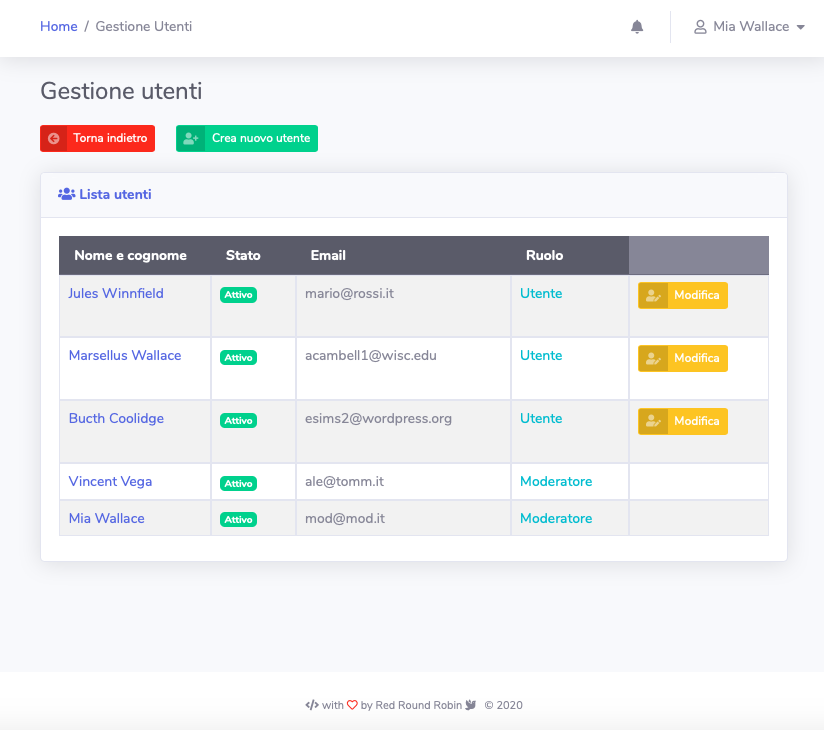
\includegraphics[scale=0.600]{res/images/mod/listaUtenti.png}
		\caption{Lista utenti}
	\end{figure}

	\subsubsection{Visualizzazione lista utenti - 0:05}
	\begin{figure}[H]
		\centering
		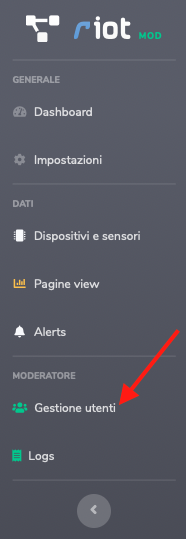
\includegraphics[scale=0.600]{res/images/mod/menuUtente.png}
		\caption{Selezione della gestione utenti dal menu}
	\end{figure}
		Come moderatore, è presente nella sidebar a sinistra un menù per la moderazione dal quale è possibile andare a gestire gli utenti del proprio ente.
		Per visualizzare la sezione, aprire il menù e cliccare su Gestione utenti.

	\subsubsection{Visualizzazione informazioni di un utente - 0:20}
		All'interno della sezione di gestione degli utenti sarà possibile visualizzare la lista degli utenti appartenenti al proprio ente con il loro relativo ruolo.
		\begin{figure}[H]
		\centering
		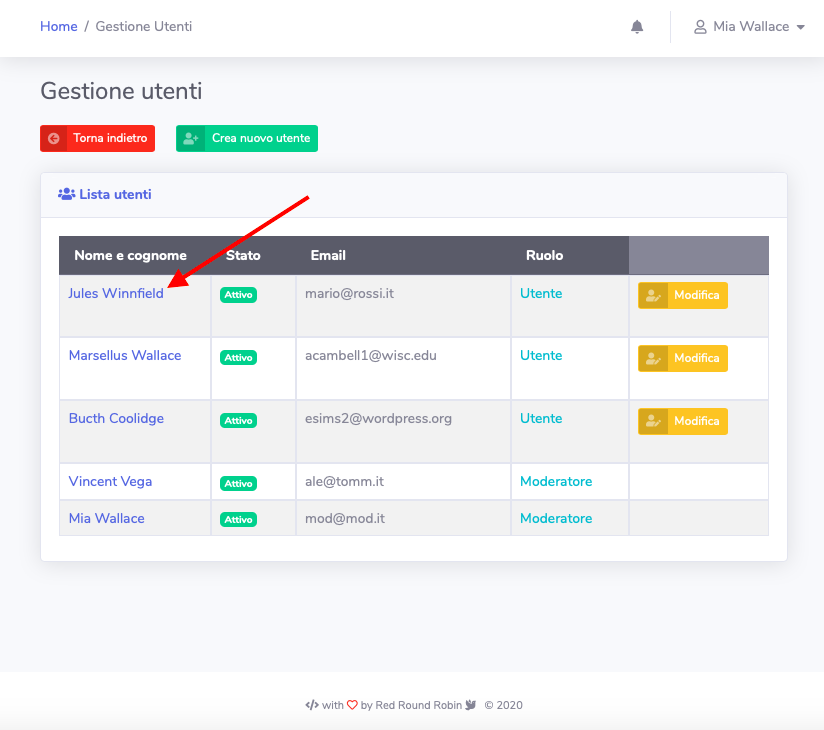
\includegraphics[scale=0.600]{res/images/mod/selUtente.png}
		\caption{Selezione di un utente}
	\end{figure}
	\begin{figure}[H]
		\centering
		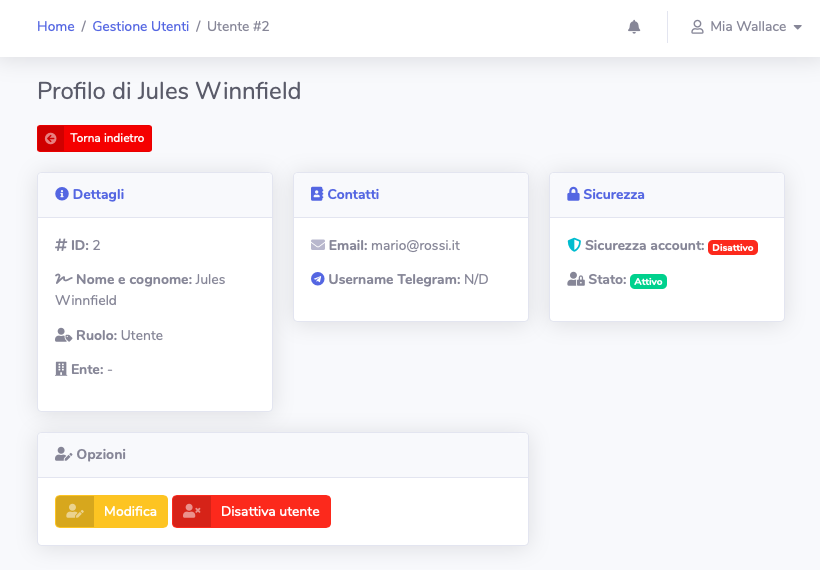
\includegraphics[scale=0.600]{res/images/mod/dettagliUtente.png}
		\caption{Dettagli di un utente}
	\end{figure}
		Cliccando sull'id degli utenti o sul loro nome sarà possibile entrare dentro il loro profilo per visualizzare maggiori informazioni utili, come i contatti e i livelli di sicurezza abilitati.

\newpage \subsection{7. Mod - Creazione e modifica utenti}

	\begin{itemize}
		\item \href{https://www.youtube.com/watch?v=PjySMOLCtMA&list=PLPKYjnuIh1FA3b3jn_bwY_ztYzaFn2mIT&index=10}{Visualizza il video tutorial su YouTube} 
	\end{itemize}

	\subsubsection{Creazione utente - 0:04}
		\begin{figure}[H]
		\centering
		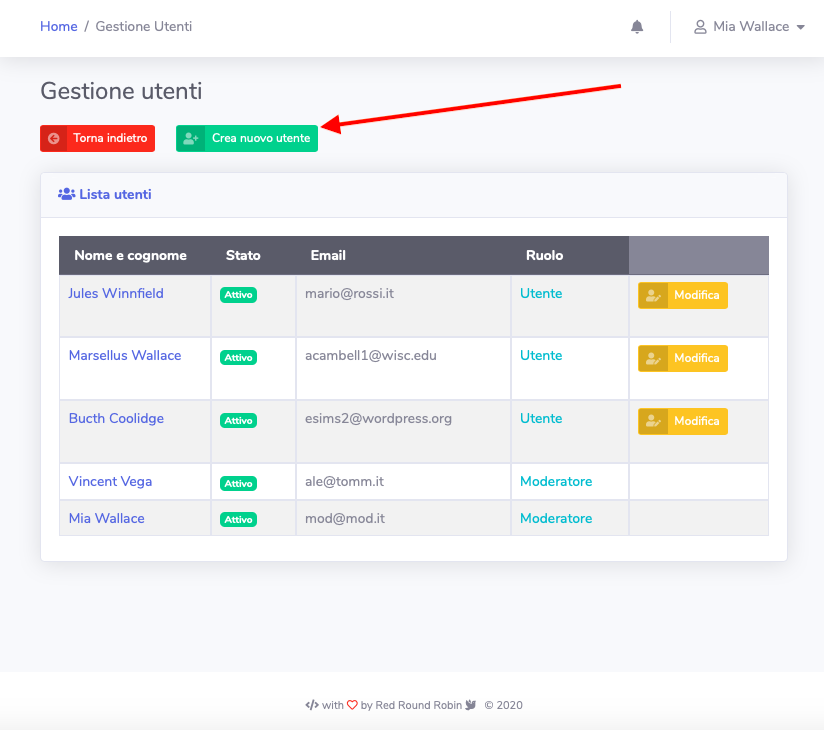
\includegraphics[scale=0.600]{res/images/mod/selCreazUtenti.png}
		\caption{Selezione della creazione di un nuovo utente}
	\end{figure}
		Per creare un utente, è necessario entrare nella gestione utente presente nella sidebar e cliccare sul bottone verde in alto (Crea nuovo utente).
		\begin{figure}[H]
		\centering
		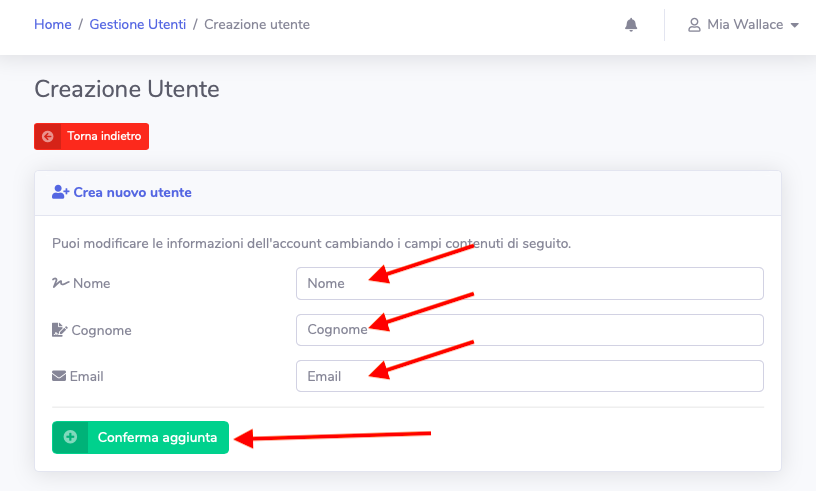
\includegraphics[scale=0.600]{res/images/mod/creazUtente.png}
		\caption{Form di creazione di un utente}
	\end{figure}
		Da qui sarà necessario compilare tutte le informazioni richieste nel form, tra cui Nome, Cognome e indirizzo email.
		Una volta compilato, cliccare sul pulsante crea utente.
		L'utente verrà quindi creato e verrà visualizzata una password associata all'utente al completamento della sua creazione. Sarà compito del moderatore comunicare la password all'utente appena creato.

	\subsubsection{Modifica utente - 0:34}
		\begin{figure}[H]
		\centering
		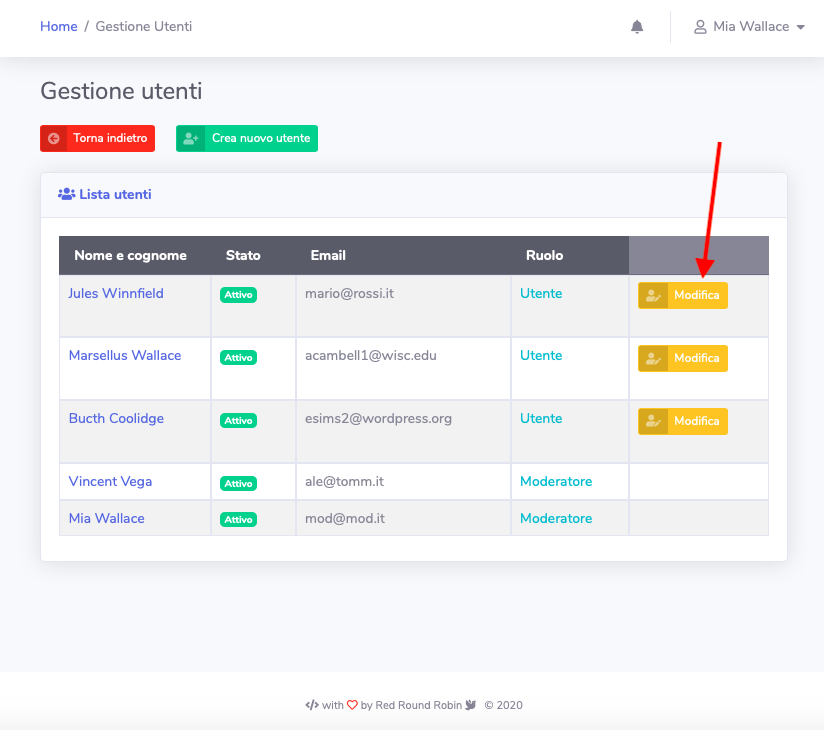
\includegraphics[scale=0.600]{res/images/mod/selModUtente.png}
		\caption{Selezione della modifica di un utente}
	\end{figure}
	\begin{figure}[H]
		\centering
		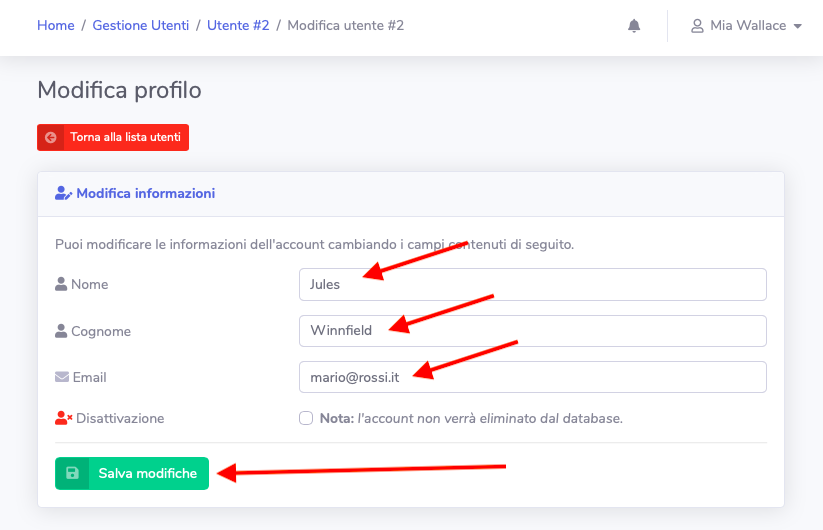
\includegraphics[scale=0.600]{res/images/mod/modUtente.png}
		\caption{Form di modifica di un utente}
	\end{figure}
		Il profilo di potrà essere modificato premendo il bottone giallo Modifica, presente sia dentro il profilo che nella tabella della lista utenti presente nella sezione di gestione degli utenti.
		Le informazioni modificabili sono le medesime inserite in fase di creazione, ovvero nome, cognome ed email.
		Infine è necessario premere Salva modifiche.



\newpage \subsection{8. Mod - Disattivazione e ripristino utente}

	\begin{itemize}
		\item \href{https://www.youtube.com/watch?v=PjySMOLCtMA&list=PLPKYjnuIh1FA3b3jn_bwY_ztYzaFn2mIT&index=11}{Visualizza il video tutorial su YouTube} 
	\end{itemize}

	\subsubsection{Disattivazione utente - 0:05}
		Per disattivare un utente, è necessario entrare nella gestione utenti.
		\begin{figure}[H]
		\centering
		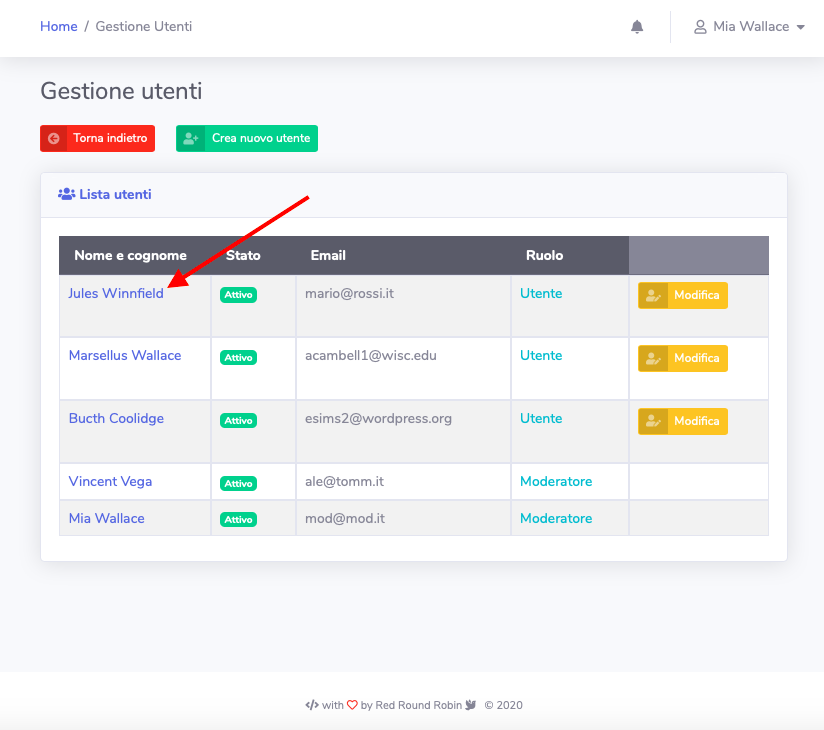
\includegraphics[scale=0.600]{res/images/mod/selUtente.png}
		\caption{Selezione di un utente}
	\end{figure}
	\begin{figure}[H]
		\centering
		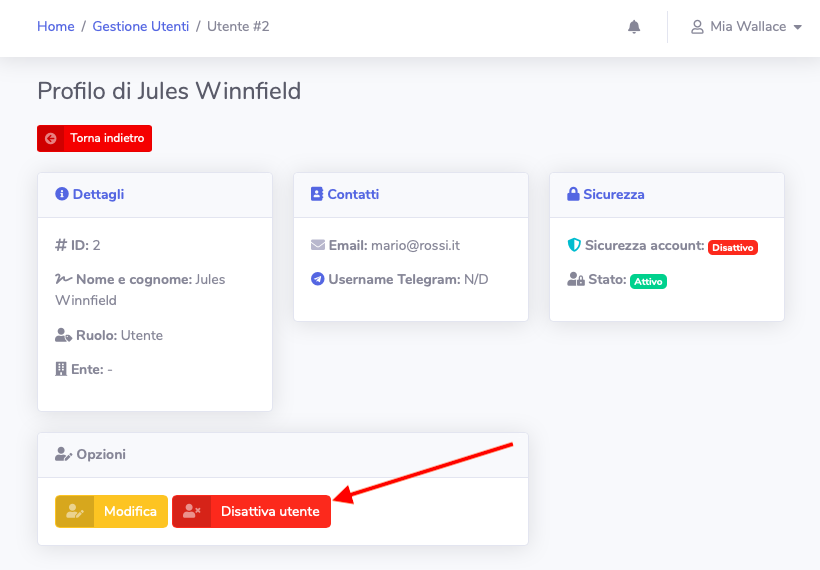
\includegraphics[scale=0.600]{res/images/mod/elimUtente.png}
		\caption{Disattivazione di un utente}
	\end{figure}
		Una volta dentro, è possibile muoversi nel profilo dell'utente e cliccare il bottone rosso Disattiva utente.
		\begin{figure}[H]
		\centering
		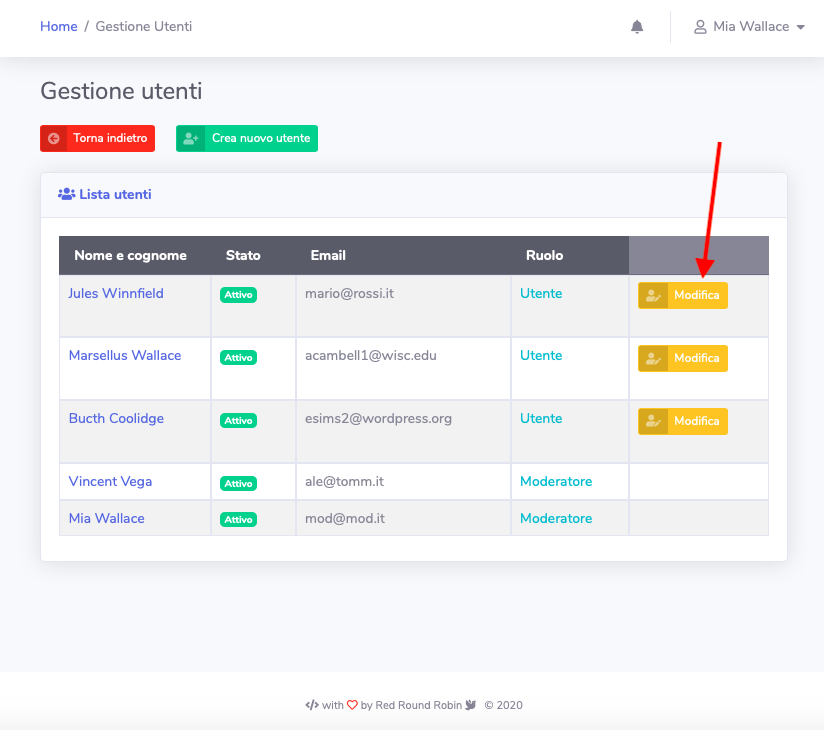
\includegraphics[scale=0.600]{res/images/mod/selModUtente.png}
		\caption{Selezione della modifica di un utente}
	\end{figure}
		\begin{figure}[H]
		\centering
		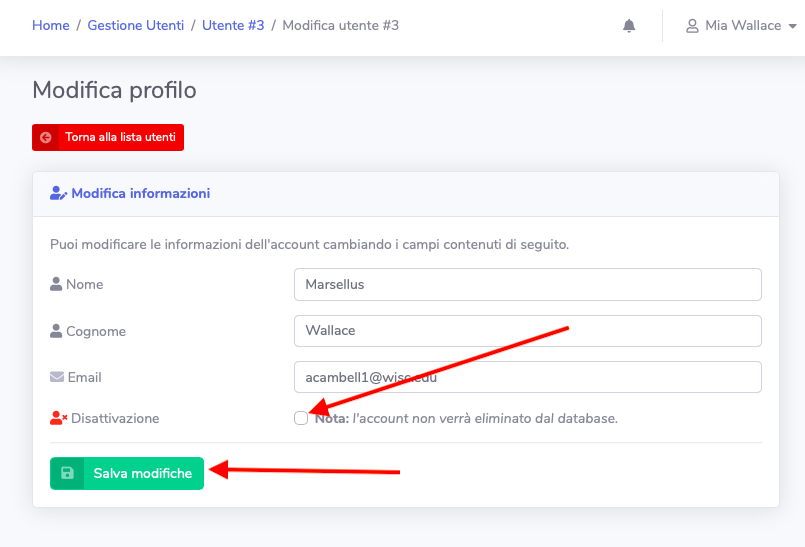
\includegraphics[scale=0.600]{res/images/mod/disattUtente.png}
		\caption{Checkbox per effettuare la disattivazione di un utente}
	\end{figure}
		In alterativa è possibile effettuare la stessa operazione entrando nella modifica dell'utente, spuntando l'opzione di disattivazione e cliccando il bottone per il salvataggio delle modifiche. 
		\begin{figure}[H]
		\centering
		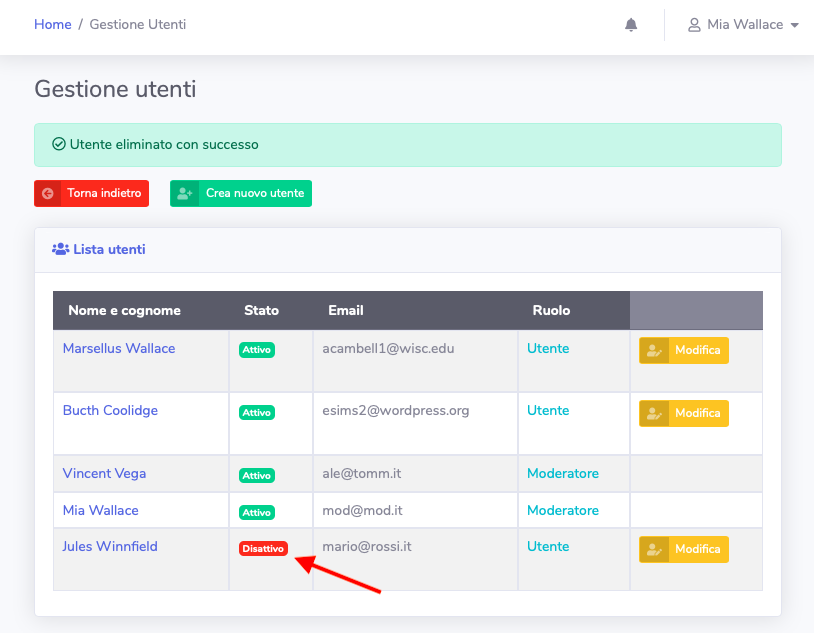
\includegraphics[scale=0.600]{res/images/mod/utenteDisatt.png}
		\caption{Lista degli utenti con utente disattivato}
	\end{figure}
		L'utente verrà quindi disattivato, come è possibile vedere dalla tabella. Un utente disattivato non potrà accedere alla webapp e non potrà usare il bot Telegram.

	\subsubsection{Ripristino utente - 0:30}
		\begin{figure}[H]
		\centering
		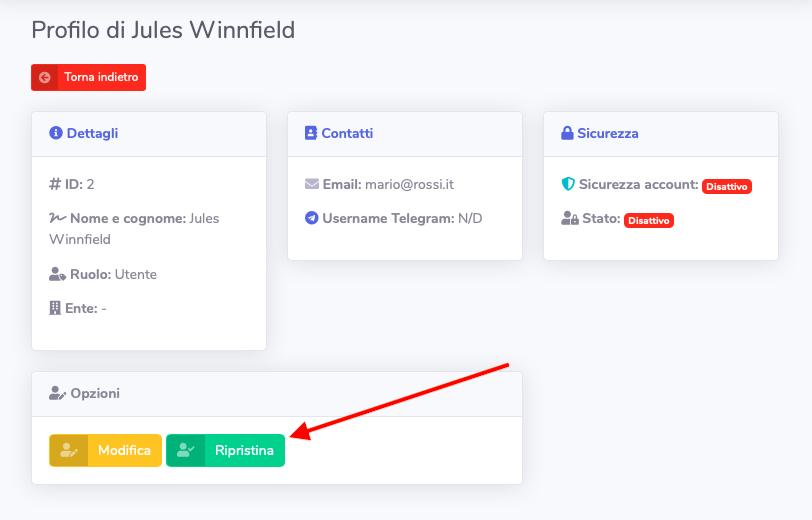
\includegraphics[scale=0.600]{res/images/mod/ripristUtente.png}
		\caption{Ripristino di un utente disattivato}
	\end{figure}
		Per riattivare un utente sarà sufficiente navigare fino al suo profilo (seguendo quanto spiegato nella sezione \textbf{Visualizzazione informazioni di un utente}) e cliccare il bottone verde Ripristina.
		\begin{figure}[H]
		\centering
		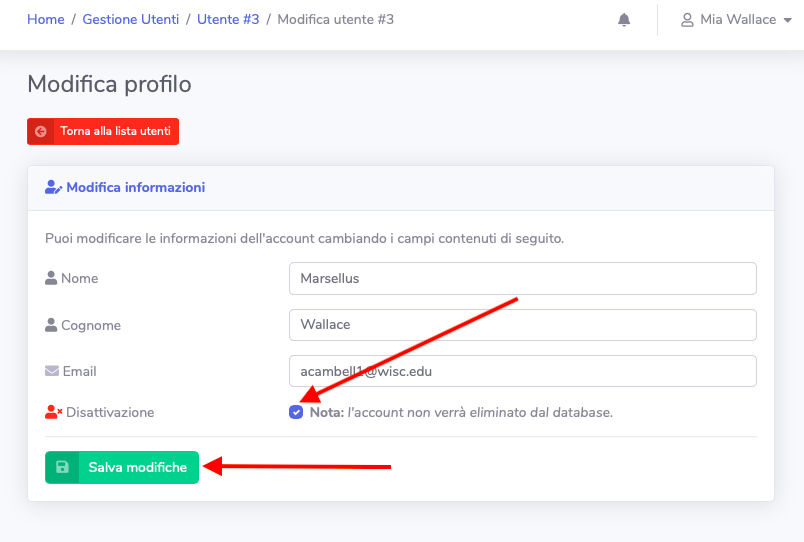
\includegraphics[scale=0.600]{res/images/mod/ripristUtente1.png}
		\caption{Metodo alternativo per ripristinare un utente}
	\end{figure}
		Alternativamente è possibile ripristinare un utente togliendo la spunta da Disattivazione all'interno del form di modifica dell'utente. Infine è necessario premere il bottone Salva Modifiche.


\newpage \subsection{9. Mod - Gestione degli alerts}
	
	\begin{itemize}
		\item \href{https://www.youtube.com/watch?v=PjySMOLCtMA&list=PLPKYjnuIh1FA3b3jn_bwY_ztYzaFn2mIT&index=12}{Visualizza il video tutorial su YouTube} 
	\end{itemize}

	\begin{figure}[H]
		\centering
		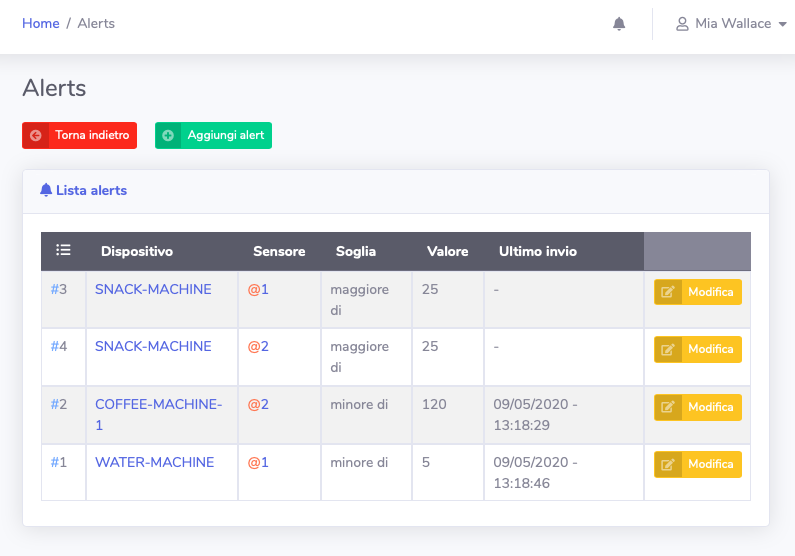
\includegraphics[scale=0.600]{res/images/mod/listaAlerts.png}
		\caption{Lista con gli alert attivi per il proprio ente}
	\end{figure}

	\subsubsection{Visualizzazione lista alert - 0:05}
		\begin{figure}[H]
		\centering
		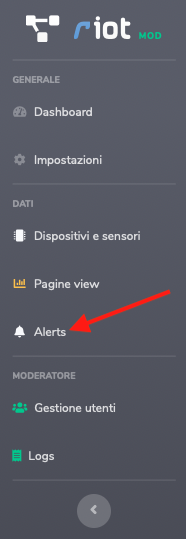
\includegraphics[scale=0.600]{res/images/mod/menuAlert.png}
		\caption{Selezione della gestione alert dal menù}
	\end{figure}
		Come moderatori, è possibile gestire gli alerts del proprio ente.
		Per fare ciò entrare nella sezione alerts dalla sidebar in cui si potranno visualizzare tutte le informazioni per gli alert del proprio ente. 
		Una volta dentro, sarà possibile inoltre aggiungere, modificare o eliminare un alert.

	\subsubsection{Creazione alert - 0:15}
	\begin{figure}[H]
		\centering
		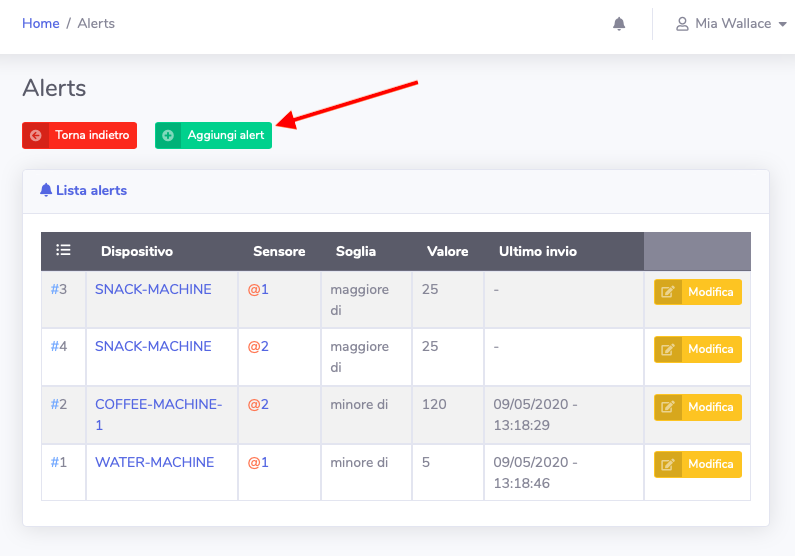
\includegraphics[scale=0.600]{res/images/mod/selCreazAlert.png}
		\caption{Selezione della creazione di un nuovo alert}
	\end{figure}
		Per creare un alert è necessario entrare nella sezione di gestione degli alert e cliccare sul bottone Aggiungi alert posto sopra la tabella.
		\begin{figure}[H]
		\centering
		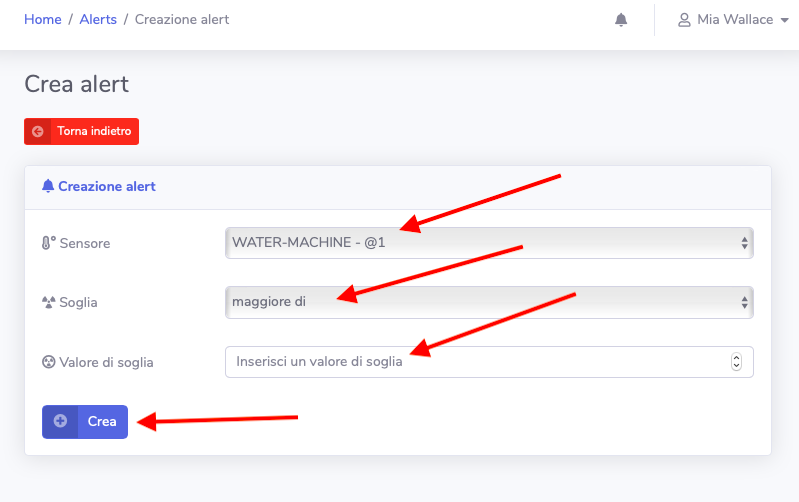
\includegraphics[scale=0.600]{res/images/mod/creazAlert.png}
		\caption{Form di creazione di un alert}
	\end{figure}
		Una volta dentro, selezionare il sensore di cui si vuole ricevere un alert al superamento della soglia. Selezionare quindi la soglia e il valore di soglia.
		Dopo aver premuto il bottone Crea, l'alert verrà quindi aggiunto e sarà visualizzabile nella tabella all'interno della sezione.

	\subsubsection{Modifica alert - 0:32}
		\begin{figure}[H]
		\centering
		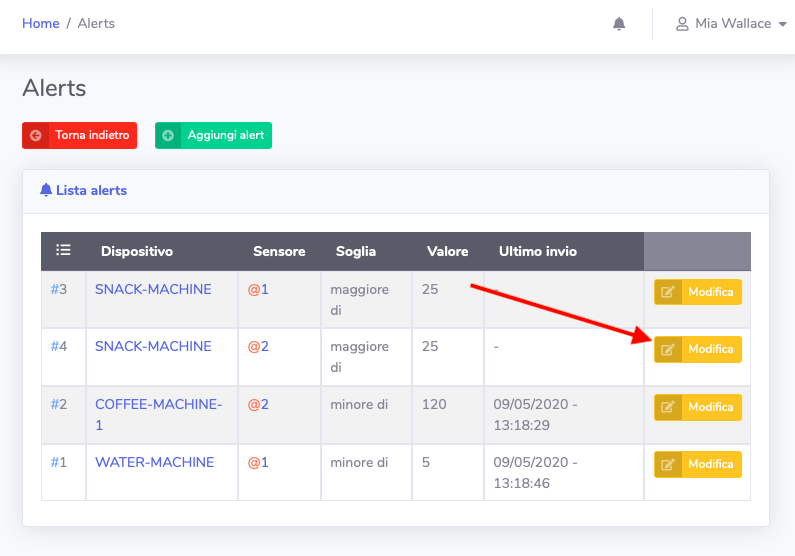
\includegraphics[scale=0.600]{res/images/mod/selModAlert.png}
		\caption{Selezione della modifica di un alert}
	\end{figure}
	\begin{figure}[H]
		\centering
		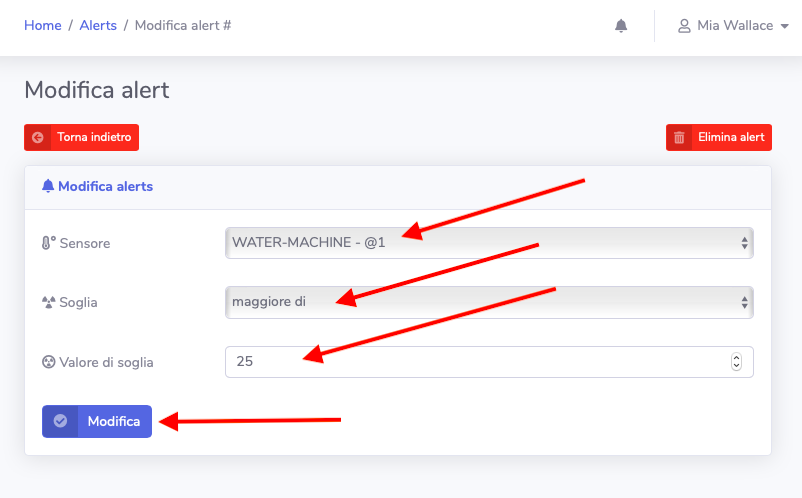
\includegraphics[scale=0.600]{res/images/mod/modAlert.png}
		\caption{Form di modifica di un alert}
	\end{figure}
		Per modificare un alert, è sufficiente cliccare il bottone Modifica presente nella tabella della sezione di gestione degli alert. Da qui sarà possibile modificare tutti i campi riportati. Infine è necessario cliccare su Modifica.

	\subsubsection{Eliminazione alert - 0:49}
	\begin{figure}[H]
		\centering
		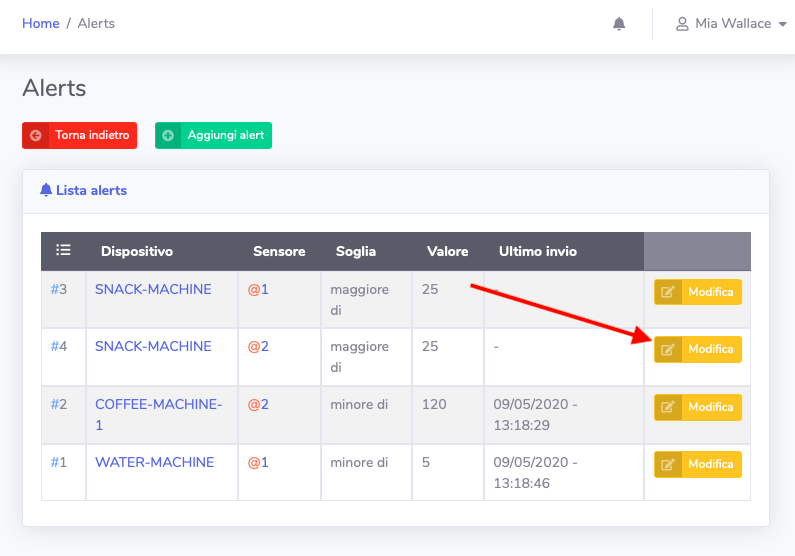
\includegraphics[scale=0.600]{res/images/mod/selModAlert.png}
		\caption{Selezione della modifica di un alert}
	\end{figure}
	\begin{figure}[H]
		\centering
		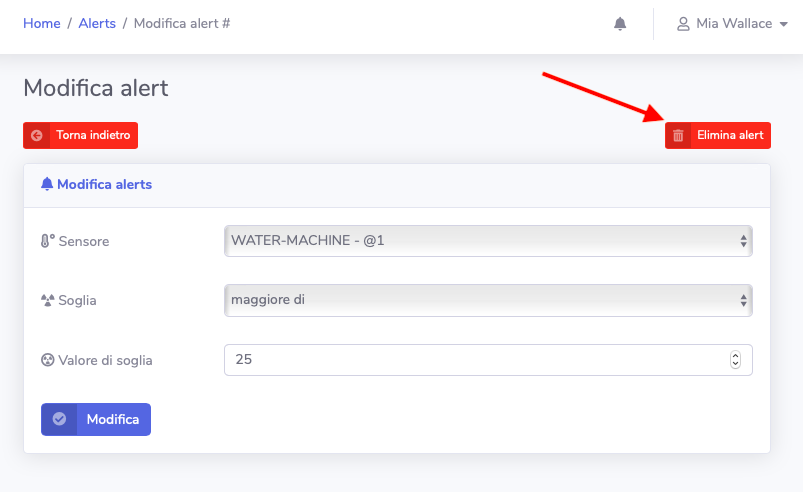
\includegraphics[scale=0.600]{res/images/mod/elimAlert.png}
		\caption{Eliminazione di un alert}
	\end{figure}
		Per eliminare un alert è sufficiente cliccare il bottone Modifica presente nella tabella della sezione di gestione degli alert e da qui sarà possibile eliminarlo premendo sul bottone Elimina alert posto in alto a destra sulla pagina.
	

\newpage \subsection{10. Mod - Visualizzazione logs}
	\begin{itemize}
		\item \href{https://www.youtube.com/watch?v=PjySMOLCtMA&list=PLPKYjnuIh1FA3b3jn_bwY_ztYzaFn2mIT&index=13}{Visualizza il video tutorial su YouTube} 
	\end{itemize}
	\subsubsection{Visualizzazione logs - 0:05}
		\begin{figure}[H]
		\centering
		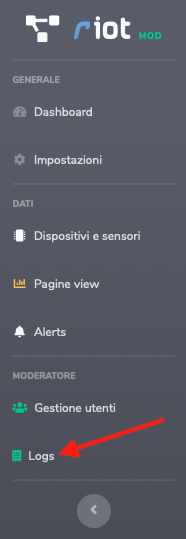
\includegraphics[scale=0.600]{res/images/mod/menuLogs.png}
		\caption{Selezione logs dal menù}
	\end{figure}
		Come moderatori è possibile visualizzare le logs di tutti i membri del proprio ente.
		Per visualizzare le logs, è sufficiente entrare da Moderazione in Logs e verrà visualizzata la tabella contenente tutte le azioni effettuate da parte degli utenti.
		\begin{figure}[H]
		\centering
		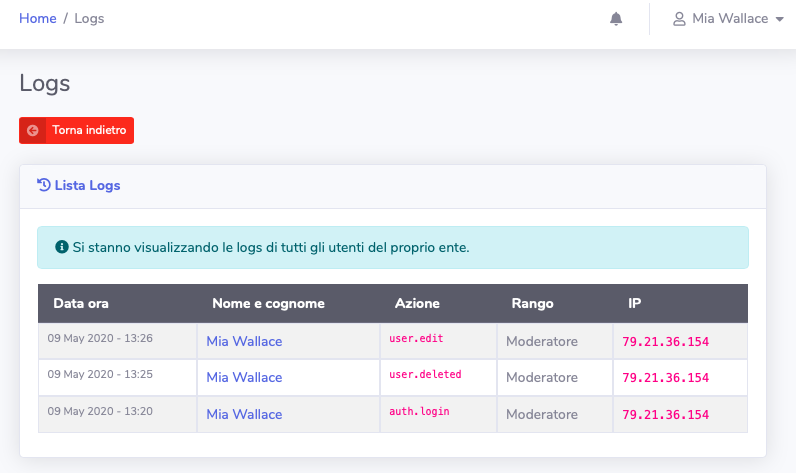
\includegraphics[scale=0.600]{res/images/mod/visLogs.png}
		\caption{Tabella delle logs registrate}
	\end{figure}
		Tra le informazioni disponibili troviamo il nome e cognome, la data ora, l’azione eseguita, il rango dell’utente e l’indirizzo Ip. 

